\section{Justificación}

La presente propuesta de proyecto busca desarrollar un videojuego análogo al clásico ``Pong" pero con una trayectoria circular, utilizando exclusivamente componentes electrónicos discretos. 
La motivación principal detrás de esta iniciativa es explorar y aplicar principios fundamentales de la electrónica analógica y digital sin depender de microcontroladores o sistemas embebidos convencionales.

El diseño de videojuegos con hardware dedicado es un área de interés tanto en la educación como en la experimentación tecnológica. 
A diferencia de las implementaciones tradicionales con microcontroladores o software, este proyecto permite un aprendizaje profundo sobre el diseño analógico y digital. 

Además, el uso de circuitos discretos brinda una oportunidad para comprender el funcionamiento interno de sistemas electrónicos sin abstraer su comportamiento mediante software. 
En el curso Laboratorio de Microcontroladores IE0624, se ha realizado una implementación del juego ``Pong" en un microcontrolador STM32 como se muestra en la \figref{uPong} (\href{https://github.com/Roger-505/ie0624/tree/main/proyecto}{$\mu$Pong}), por lo que la implementación del famosos juego utilizando componentes analógicos discretos presenta una alternativa al diseño de sistemas electrónicos, donde los dispositivos electrónicos modernos por lo general usan algún tipo de sistema incrustado en su diseño. 

\begin{figure}[H]
    \centering
    \begin{minipage}{0.45\textwidth}
        \centering
        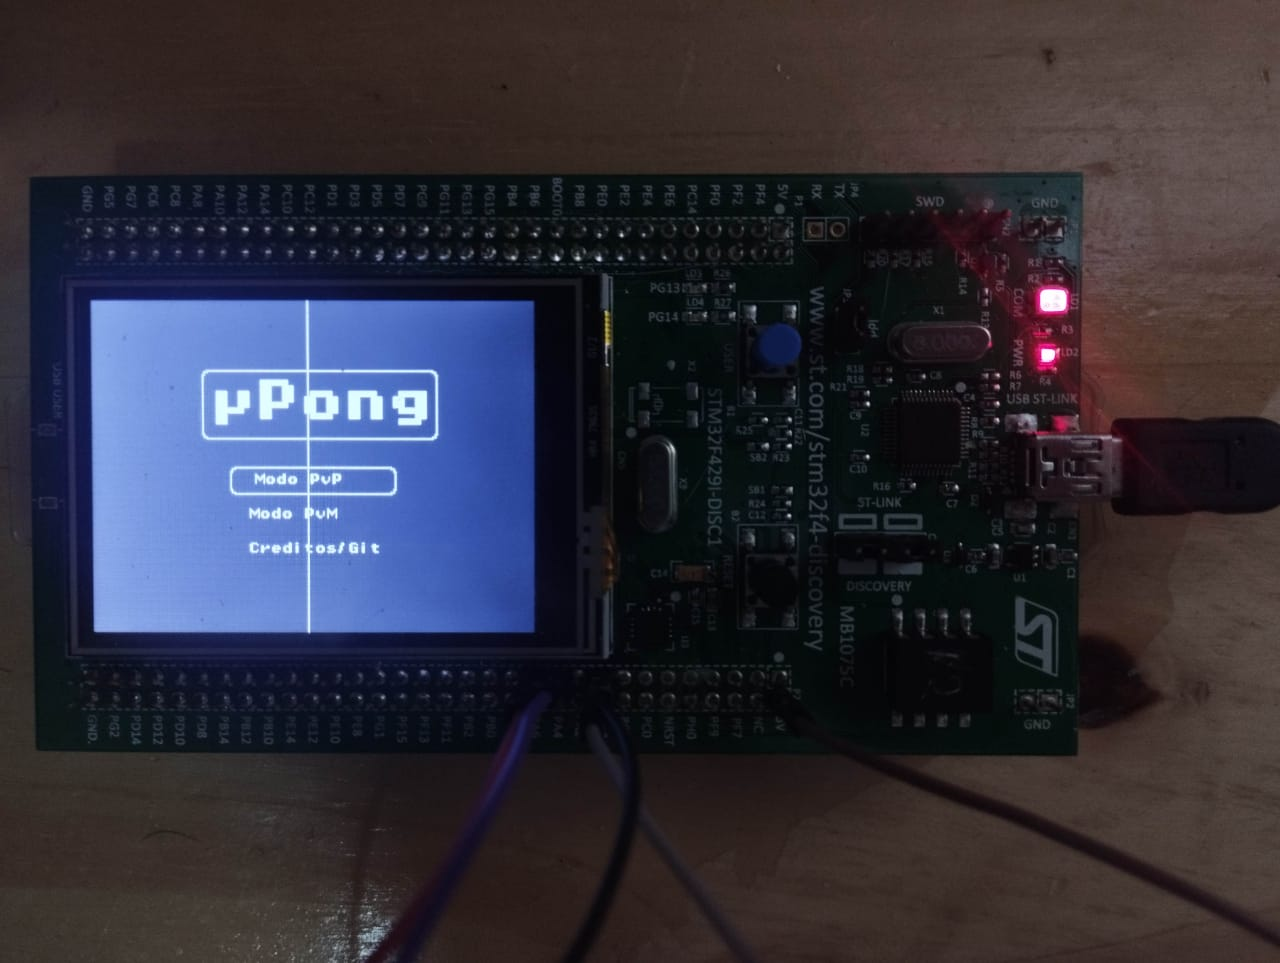
\includegraphics[width=\textwidth]{figs/justificacion/main_menu.jpeg}
        \caption*{(a): Menú Principal.}
    \end{minipage}%
    \begin{minipage}{0.45\textwidth}
        \centering
        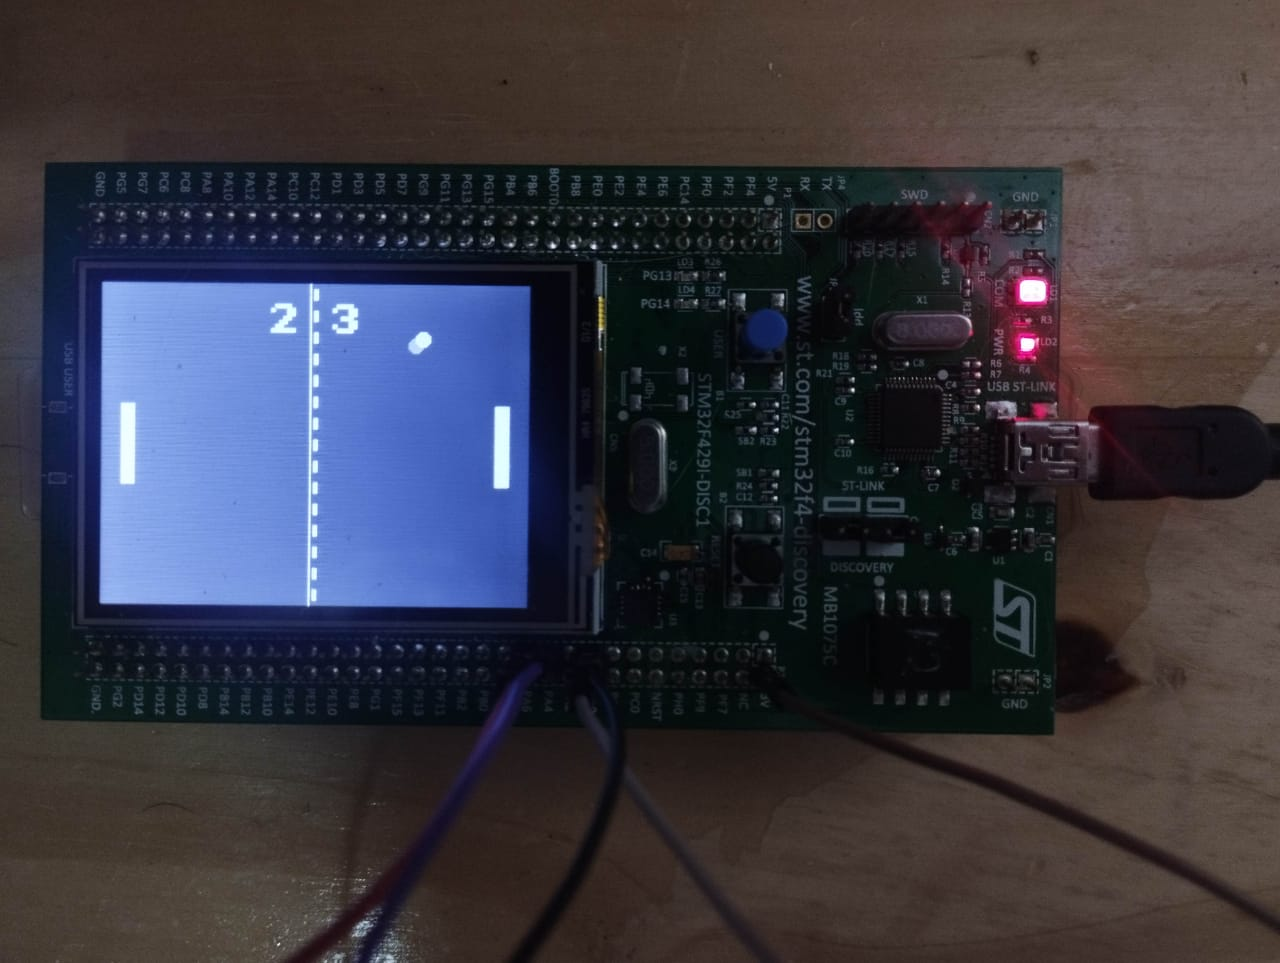
\includegraphics[width=\textwidth]{figs/justificacion/gameplay.jpeg}
        \caption*{(b): Gameplay.}
    \end{minipage}%
    \caption{Implementación del juego Pong en un microcontrolador STM32: $\mu$Pong}
    \label{uPong}
\end{figure}

Este proyecto integra múltiples áreas de la electrónica, incluyendo:
\begin{itemize}
    \item \textbf{Electrónica Analógica}: Generación de señales y sincronización utilizando osciladores en cuadratura con amplificadores operacionales.
    \item \textbf{Electrónica Digital}: Implementación de la lógica del juego mediante compuertas lógicas y flip-flops para el control de la pelota y detección de colisiones.
    \item \textbf{Procesamiento de Señales}: Modulación de señales para la representación gráfica del juego en la pantalla de un osciloscopio. 
\end{itemize}

El proyecto ``Round Pong" no solo tiene un valor recreativo, sino que también actúa como una plataforma de aprendizaje para la experimentación con hardware. 
Puede servir como un recurso didáctico para ejemplificar lo que se puede lograr por medio del diseño electrónico, así como presentar un uso práctico de una variedad de topologías de circuitos que utilizan amplificadores operacionales.